\subsection{O Método Sweby}

O método Sweby é um método do tipo TVD (Total Variation Diminishing) que utiliza um limitador para evitar oscilações não físicas em regiões de alta variação. O limitador Sweby é ajustável por meio do parâmetro \(\beta\), permitindo balancear precisão e dissipação numérica \cite{sweby1984high}.

A equação geral para o fluxo numérico utilizando o limitador Sweby é dada por:

\begin{equation}
    \phi_{\text{lim}} = \max\left(0, \min\left(\beta \theta, \min\left(1, \theta\right)\right)\right),
\end{equation}

onde \(\theta\) é o gradiente relativo entre as células adjacentes, e \(\beta\) é o parâmetro de controle do limitador, comumente usado como \(\beta = 1,5\).

A equação do método TVD aplicado ao método Sweby é expressa como:

\begin{equation}
    Q_i^{n+1} = Q_i^n - C (F_{i+1/2} - F_{i-1/2}),
\end{equation}

onde os fluxos \(F_{i+1/2}\) e \(F_{i-1/2}\) são calculados com base no limitador Sweby.

\begin{figure}[H]
    \centering
    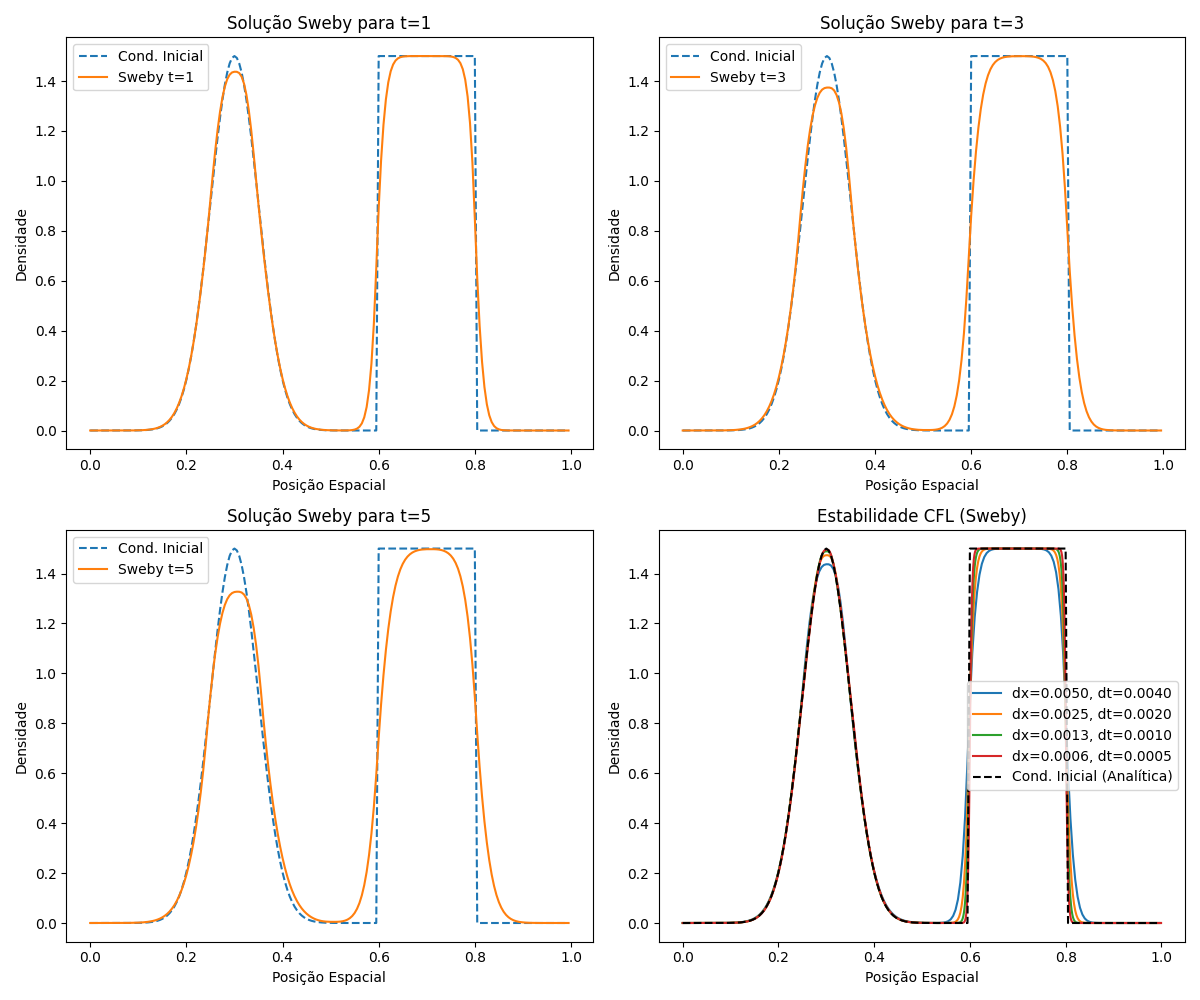
\includegraphics[width=\textwidth]{code/images/Sweby.png}
    \caption{Solução Sweby para \(t=1\), \(t=3\) e \(t=5\), com a condição inicial representada pela linha tracejada.}
    \label{fig:sweby}
\end{figure}

\begin{table}[H]
    \centering
    \begin{tabular}{rrrrrr}
\toprule
Posicao Espacial & Condicao Inicial & Sweby t=1 & Sweby t=3 & Sweby t=5 & Posicao da Estabilidade \\
\midrule
0.000000 & 0.000000 & 0.000000 & 0.000002 & 0.000006 & 0.000000 \\
0.050000 & 0.000006 & 0.000012 & 0.000034 & 0.000053 & 0.050000 \\
0.100000 & 0.000503 & 0.000718 & 0.001223 & 0.001420 & 0.100000 \\
0.150000 & 0.016663 & 0.018961 & 0.023321 & 0.022593 & 0.150000 \\
0.200000 & 0.203003 & 0.206288 & 0.213317 & 0.192373 & 0.200000 \\
0.250000 & 0.909796 & 0.923582 & 0.967856 & 0.912867 & 0.250000 \\
0.300000 & 1.500000 & 1.437160 & 1.373804 & 1.325958 & 0.300000 \\
0.350000 & 0.909796 & 0.904268 & 0.930223 & 1.030586 & 0.350000 \\
0.400000 & 0.203003 & 0.208248 & 0.218056 & 0.261015 & 0.400000 \\
0.450000 & 0.016663 & 0.019849 & 0.025923 & 0.037466 & 0.450000 \\
0.500000 & 0.000503 & 0.000766 & 0.001917 & 0.004691 & 0.500000 \\
0.550000 & 0.000006 & 0.003678 & 0.028017 & 0.040087 & 0.550000 \\
0.600000 & 1.500000 & 0.890163 & 0.860449 & 0.740881 & 0.600000 \\
0.650000 & 1.500000 & 1.497814 & 1.475949 & 1.438465 & 0.650000 \\
0.700000 & 1.500000 & 1.500000 & 1.499627 & 1.497384 & 0.700000 \\
0.750000 & 1.500000 & 1.498258 & 1.481938 & 1.472013 & 0.750000 \\
0.800000 & 1.500000 & 0.849292 & 0.804179 & 0.905699 & 0.800000 \\
0.850000 & 0.000000 & 0.004615 & 0.036054 & 0.083578 & 0.850000 \\
0.900000 & 0.000000 & 0.000001 & 0.000308 & 0.002432 & 0.900000 \\
0.950000 & 0.000000 & 0.000000 & 0.000003 & 0.000025 & 0.950000 \\
\bottomrule
\end{tabular}

    \caption{Tabela de resultados para o método Sweby nas posições espaciais selecionadas e diferentes tempos.}
    \label{tab:sweby}
\end{table}

\subsection{Análise dos Resultados do Método Sweby}

A Figura~\ref{fig:sweby} apresenta os resultados obtidos com o método Sweby nos instantes \(t=1\), \(t=3\) e \(t=5\). Para \(t=1\), a solução mantém o perfil da condição inicial com alta precisão, preservando os gradientes e evitando oscilações. Nos tempos \(t=3\) e \(t=5\), observam-se pequenas alterações na amplitude das regiões de alta variação, porém sem oscilações significativas, evidenciando a eficácia do limitador Sweby em controlar oscilações enquanto mantém uma boa precisão.

\subsection{Implementação em Python}

O código em Python para o método Sweby utiliza a função principal \texttt{resolverAdveccaoTVD}, que aplica o limitador e calcula a evolução da densidade ao longo do tempo, conforme mostrado na Listagem~\ref{lst:codigo_sweby}. A implementação do limitador Sweby é dada por:

\begin{lstlisting}[language=Python, caption={Código para resolver a advecção usando o método Sweby}, label={lst:codigo_sweby}]
def limitadorSweby(theta, beta=1.5):
    return np.maximum(0, np.minimum(beta * theta, np.minimum(1, theta)))

def metodoTvdSweby(densidade, nt, intervaloTempo, intervaloEspacial, numeroCourant):
    """
    Método TVD para resolver a advecção utilizando o limitador de Sweby.
    """
    for n in range(nt):
        novaDensidade = densidade.copy()
        for i in range(len(densidade)):
            esquerda = (i - 1) % len(densidade)
            direita = (i + 1) % len(densidade)
            # Calcula o gradiente relativo (theta)
            theta = (densidade[i] - densidade[esquerda]) / (densidade[direita] - densidade[i] + 1e-6)
            # Fluxos para direita e esquerda
            fluxoDireita = densidade[i] + 0.5 * numeroCourant * (1 - numeroCourant) * limitadorSweby(theta) * (densidade[direita] - densidade[i])
            fluxoEsquerda = densidade[esquerda] + 0.5 * numeroCourant * (1 - numeroCourant) * limitadorSweby(theta) * (densidade[i] - densidade[esquerda])
            # Atualiza a densidade
            novaDensidade[i] = densidade[i] - numeroCourant * (fluxoDireita - fluxoEsquerda)
        densidade = novaDensidade.copy()
    return densidade
\end{lstlisting}

A implementação do método Sweby garante estabilidade e precisão ao controlar oscilações em gradientes acentuados. O número de Courant \(C=0,8\) é usado para calcular o fluxo numérico em cada interface, assegurando a convergência da solução.
